\chapter{Analysis of Posteriors and Inference by Enumeration} \label{chap:4}
In a model as complex as a generative scene graph program, it becomes essential to carefully check and analyze the behavior of the posterior to ensure it is a good representation of the data.
This chapter describes a set of synthetic experiments that carefully inspect isolated aspects of the model to ensure their posteriors exhibit reasonable behavior that conforms to intuition.

\section{Enumerative inference}
In conducting an analysis of a generative scene graph program, it is useful to inspect the posterior distribution induced by constraining some subset of the model.
Calculating the full posterior is intractable (indeed, this is why inference is necessary in the first place).
However, if most of the model's latent variables are constrained, it's reasonable to enumerate over a small set of free variables, and calculate a normalized density for a range of their values, which is a close approximation to the posterior conditioned on the constrained variables.
Note that this approach is limited in its ability to examine interactions between variables, and in generality the posterior conditioned on just the observed neural pose detections can behave radically differently from the posterior generated by constraining most of the model.
Nonetheless, this chapter shows that these projections can still be a rich source of information for understanding and improving scene graph priors, especially model hyperparameters.

\section{Structure posterior} \label{section:structureAnalysis}
This section looks at the model's predictions for structure between objects, as a function of the observed vertical offset $y$ between their closest faces.
The analysis conducted considers the static model and dynamic model respectively, and looks at the behavior of the structure posterior under multiple settings of model hyperparameters.
It ultimately demonstrates the high variability of the posterior's qualitative behavior with respect to hyperparameters; this in turn shows the vital importance of proper hyperparameter tuning in ensuring the correctness of scene graph models.
\begin{figure}[h]
  \centering
  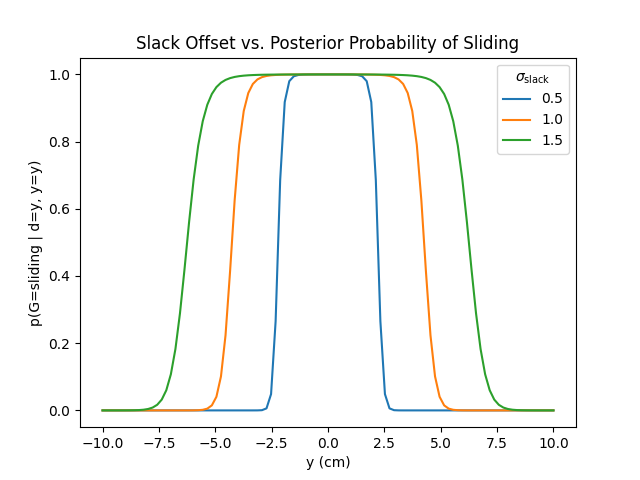
\includegraphics[width=0.9\columnwidth]{posStructurePosterior}
  \caption{
    Probability that an object is sliding in a static scene with different settings of $\sigma_\mathrm{slack}$, and observed/latent vertical offset $y$.
  }
  \label{fig:posStructurePosterior}
\end{figure}

\subsection{Static model}
An experimental scene was created with two objects, in order to visualize the enumerated structure posterior for $G$, given an observed one-dimensional vertical offset $y$ between the object's closest faces.
In the model, $y$ also denotes the vertical gap in the observed object's faces, $d$ denotes the sliding object's \textit{slack offset}, with prior $p_\mathrm{norm(0, \sigma_\mathrm{slack})}(d)$ where $\sigma_\mathrm{slack}$ is the hyperparameter for the slack prior (see~\ref{section:slack} for a reminder of the slack variable model in sliding contacts).
The latent parameters are restricted to be the same as the observed poses, and the observed poses of the objects are also taken to be the same, except for their one-dimensional offset $y$.
The structure prior is uniform, so all structures have equal prior probability.

Figure~\ref{fig:posStructurePosterior} shows the posterior probability that $G$ is in a ``sliding'' configuration, given an offset $y$, for a few different settings of $\sigma_\mathrm{slack}$.
Predictably, the wider the distribution on slack, the larger a gap the model is willing to allow while still classifying the objects as ``sliding''.
Note the relatively sharp transition in the sliding probability from almost 0 to almost 1, at a discrete cutoff point; later it's discussed if this could be a result of a poor model for the slack variable.

\raggedbottom
\pagebreak
\flushbottom

\begin{figure}[H]
  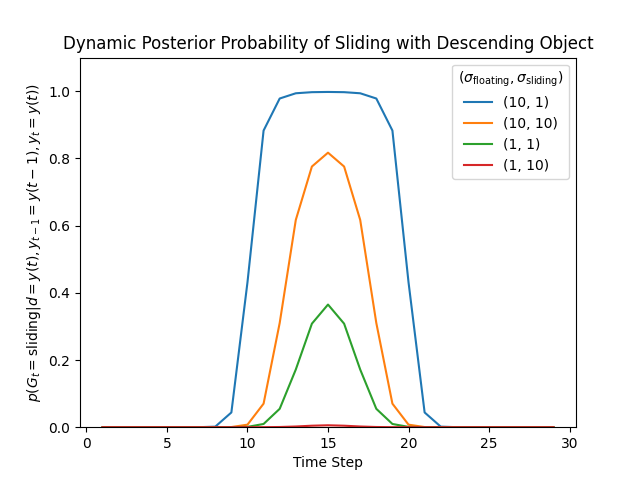
\includegraphics[width=\columnwidth]{dynamicStructurePosterior}
  \caption{
    Probability that the scene structure $G_t$ is in a ``sliding'' configuration at time $t$, in a dynamic scene where the object's observed position and slack offset is given by $y(t) = 10 - 0.67\cdot t$ cm, with hyperparameters $(\sigma_\mathrm{floating}, \sigma_\mathrm{sliding})$.
  }
  \label{fig:dynamicStructurePosterior}
\end{figure}

\subsection{Dynamic model}
The second experimental scene is very similar to the first, except for the introduction of a dynamic element to examine the effect of the dynamics parameters.
Across 30 time steps, the top object (and its observation) is lowered along $y$ from 10 cm above the bottom object, to 10 cm interpenetrating with the bottom object.
For simplicity, the prior structure is once again uniform at each time step, and thus temporally independent.
Let $\sigma_\mathrm{slack} = 1$ cm, and let the floating position dynamics be a 3D normal distribution with standard deviation $\sigma_\mathrm{floating}$, while the sliding dynamics are a 2D normal distribution with standard deviation $\sigma_\mathrm{sliding}$.

Figure~\ref{fig:dynamicStructurePosterior} shows the posterior probability that $G_t$ is in a ``sliding'' configuration, given the observed/latent offset $y$, for each time step $t$ of the dynamic scene.
Adding dynamics has added completely new behavior to the structure posterior, dependent on the additional hyperparameters.
The pose displacement is always $-0.67$ cm every time step, which is smaller than all values tested for $\sigma_\mathrm{floating}$ and $\sigma_\mathrm{sliding}$, implying that the most accurate dynamics model in this figure is the one with the tightest distribution.
The change in posterior probability in sliding structure is a consequence of the Bayesian Occam's Razor; the posterior probability for sliding is greatest (blue curve) when the sliding dynamics model is much more confident (concentrated) than the floating dynamics model, and is least in the opposite case (red curve).
This is the first instance with the Bayesian Occam's Razor adding complications to the development of scene graph models, but there are additional cases where the concentration of different branches of the model has a huge impact on the behavior of the posterior.

\begin{figure}[H]
  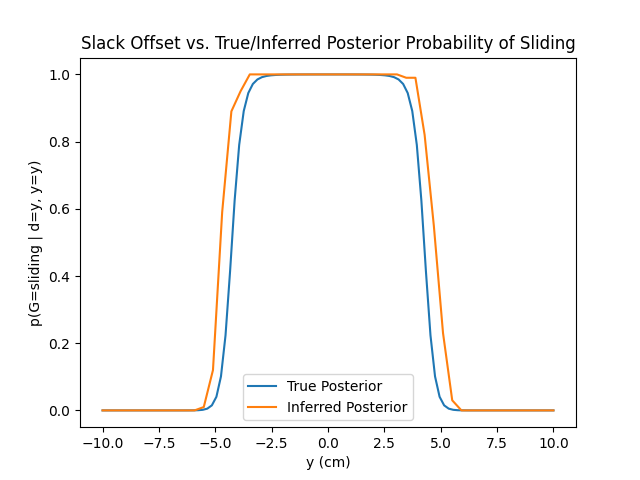
\includegraphics[width=\columnwidth]{inferredStructurePosterior}
  \caption{
    RJMCMC structure inference results.
    For each value of $d$, the approximate probability of the top object sliding is inferred as the average structure of 100 particles run with 3 iterations of the reversible jump moves applied to the top object.
  }
  \label{fig:inferredStructurePosterior}
\end{figure}

\subsection{RJMCMC structure inference}
This section includes a brief comparison of the RJMCMC structure inference procedure to the enumerated posterior.
This experiment replicates the scenario shown in Figure~\ref{fig:posStructurePosterior} with $\sigma_\mathrm{slack} = 1$ cm, and compares the performance of the inferred posterior probability of a sliding structure.
The figures shows RJMCMC accurately recovers the posterior in this situation, which is a successful first test of the correctness of the algorithmic implementation of structure inference on scene graphs.

\section{Contact slack model}
The second analysis conducted examines the enumerated posterior over the slack offset $d$.
Having a sensible posterior for slack variables is important for having a reasonable model over structure; if the slack model provides a poor explanation for any observed gap between ``contacting'' objects, the structured model will also provide a poor explanation for the scene, artificially boosting the probability the model assigns to floating structures.
Recall the prior model over slack is $p_\mathrm{slack}(d) = p_\mathrm{norm(0,\sigma_\mathrm{slack})}(d)$.

\subsection{Varying the gap between sliding objects}
A similar scene to the previous section is constructed with two objects, to visualize the enumerated slack offset posterior for $d$, given a fixed sliding structure.
The objects are again restricted to share the same observed pose, except for a one-dimensional vertical offset $y$ between their contacting faces, but the latent offset $d$ in their continuous parameters is left free (we enumerate over this instead).
In the prior model let $\sigma_\mathrm{slack} = 1$ cm, and let $p_\mathrm{inlier} = 1$.
Denote the density over the observed vertical offset $x$ as $p_\mathrm{obs}(x | y) = p_\mathrm{norm(y,\sigma_\mathrm{inlier})}(x)$, and let $\sigma_\mathrm{inlier} = 0.5$ cm.
Figure~\ref{fig:slackOffsetPosterior} shows the posteriors corresponding to various settings of the observed offset $y$.
Because the density $p(d | G=\mathrm{sliding}, y=y) = p_\mathrm{obs}(d | y=y) \cdot p_\mathrm{slack}(d)$ is a product of normal distributions, the posterior is also a normal distribution, with mean located in-between the means of the two modeling distributions.
This implies the most probable gap between two objects given a sliding structure is counter-intuitively in-between 0 and the observed gap $y$; this may explain why there is such a sharp cutoffs in the probability of a sliding structure in Figures~\ref{fig:posStructurePosterior} and \ref{fig:dynamicStructurePosterior}.
As the observed gap between two objects becomes larger, the model over slack offset quickly becomes a poor explanation of the observation.
A more reasonable model would place high mass around $d = y$, as this would explain the observation most accurately.

\begin{figure}[H]
  \centering
  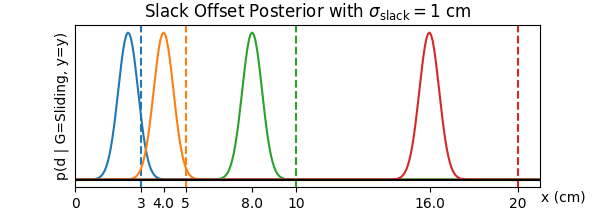
\includegraphics[width=\columnwidth]{slackOffsetPosterior}
  \caption{
    Posterior distribution on slack offset $d$.
    The dashed lines represent the set of observed $y$ values, while the curve of the same color represents the slack offset posterior, given the observed $y$ and sliding structure.
  }
  \label{fig:slackOffsetPosterior}
\end{figure}


\subsection{Hyperprior over slack standard deviation}
This section describes the addition of a hyperprior over $\sigma_\mathrm{slack}$, to more accurately allow for uncertainty in the size of the slack term.
The slack offset is now a variable sampled from an exponential distribution $\sigma_\mathrm{slack} \sample p_\mathrm{exp(0.2)}(\cdot)$ with rate parameter $\lambda = 0.2$.
Figure~\ref{fig:jointSlackHyperpriorPosterior} shows the joint posterior over $\sigma_\mathrm{slack}$ and the slack offset $d$, for an observed vertical offset $y = 5$ cm.
The figure shows that the mode of the posterior is located much closer to the observation than without a hyperprior over $\sigma_\mathrm{slack}$.
Indeed, as seen in Figure~\ref{fig:jointSlackHyperpriorPosterior}, the posterior exhibits much more reasonable behavior when letting $\sigma_\mathrm{slack} = \sigma_\mathrm{slack}^*$.
This analysis thus concludes that adding a hyperprior over slack is a viable way to increase the accuracy of the model with a sliding structure, especially when the observed gap between objects is large.
\begin{figure}[H]
  \centering
  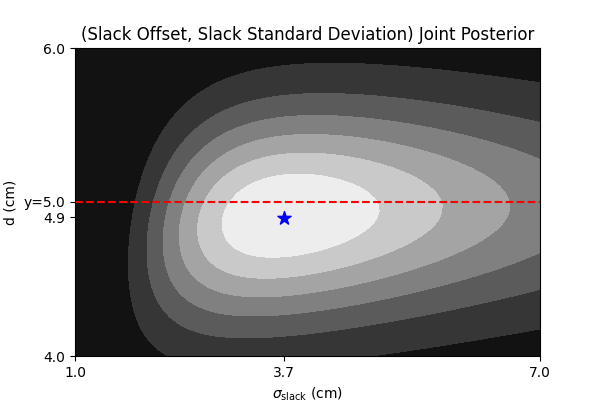
\includegraphics[width=\columnwidth]{jointSlackHyperpriorPosterior}
  \caption{
    Joint posterior $p(d,\sigma_\mathrm{slack} | y = 5.0)$.
    The dashed red line indicates the observed position $y = 5.0$ of the top object.
    The blue star indicates the maximum a posteriori $(\sigma_\mathrm{slack}^*, d^*)$.
  }
  \label{fig:jointSlackHyperpriorPosterior}
\end{figure}

\begin{figure}[H]
  \centering
  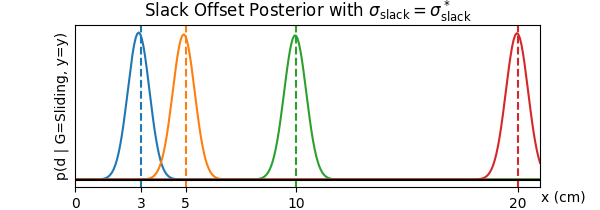
\includegraphics[width=\columnwidth]{slackOffsetPosteriorMapStdev}
  \caption{
    Slack offset posterior for $d$, conditioned on $\sigma_\mathrm{slack} = \sigma_\mathrm{slack}^*$.
    The dashed lines represent the set of observed $y$ values, while the curve of the same color represents the posterior over slack given the observed $y$ and sliding structure.
  }
  \label{fig:slackOffsetPosteriorMapStdev}
\end{figure}

\pagebreak

\section{Neural outlier model}
An essential component of the proposed scene graph model is a robust model of the output of a neural detector.
The dynamics model presented in~\ref{section:dynamics} discourages large movements in the latent poses of objects, while the prior observational model is a simple mixture of a uniform outlier distribution over poses in a finite bounded box region, with component $p(\mathrm{outlier}) = 0.1$, and a direct product of a normal and VMF inlier distribution, with component $p(\mathrm{inlier}) = 0.9$.
Ideally, the product of this model and the dynamics model would allow the scene graph model to confidently predict that large leaps in the latent position over a single time step are less probable than that specific observation being an outlier ``flicker'' detection, sampled randomly within the scene.

Figure~\ref{fig:outlierModel} shows a scene in which an object's observed pose jumps from a latent position at the origin, $x_1 = 0$, to one located a distance $y_2$.
On the left, when the dynamics and observational model are equivalent width, the posterior predicts that the detection is more likely to be an outlier than not at around $y_2 = 9.6$ cm.
On the right, when the dynamics is significantly more broad than the observational model, the posterior predicts that the detection is more likely to be an inlier, all the way up to $50$ cm $= 5\sigma_\mathrm{floating}$ away from the previous position.
The prior probability that an object travels a distance greater than $5\sigma_\mathrm{floating}$ away from the mean is less than $5.73e-7$, which is dramatically less than the prior probability of an object being an outlier $p(\mathrm{outlier}) = 0.1$.

The model on the right is counter-intuitively predicting that the object made an extraordinarily unlikely jump.
If we examine the log probability density functions evaluated at the modes of the latent pose joint distributions, for the outlier and inlier models respectively, we begin to see why:
\begin{align*}
  \log p(x_2 = 0, y_2 = 50, \mathrm{outlier} | x_1 = 0) &= \\
  \log p(\mathrm{outlier}) &+ \\
  \mathcolor{blue}{\log p(x_2 = 0 | x_1 = 0, \mathrm{outlier})} &+ \\
  \log p(y_2 = 50 | \mathrm{outlier}) &= \\
  -2.303 + \mathcolor{blue}{10.717} - (3\cdot0. + 2.289) &= 6.125 \\
  \log p(x_2 = 50, y_2 = 50, \mathrm{inlier} | x_1 = 0) &= \\
  \log p(\mathrm{inlier}) &+ \\
  \log p(x_2 = 50 | x_1 = 0, \mathrm{inlier}) &+ \\
  \mathcolor{red}{\log p(y_2 = 50 | x_1 = 0, x_2 = 50, \mathrm{inlier})} &= \\
  -0.105 - 1.783 + \mathcolor{red}{17.625} &= 15.737
\end{align*}

The dynamics model's density (blue) weights heavily in favor of the observation being an outlier.
However, the inlier pose density (red) is so tightly concentrated compared to the outlier pose model, that it dominates the calculation of the overall model weight.
The posterior tells us that the model would rather have the latent pose make an incredibly unlikely jump, if it means it can explain the observed pose confidently using the inlier observational model.
This is another occurrence of the Bayesian Occam's Razor, where the most concentrated component of the model (in this case the observation model), determines where the majority of the posterior mass is distributed.

\raggedbottom

\pagebreak

\flushbottom

\begin{figure}[H]
  \captionsetup[subfigure]{justification=centering}
  \begin{subfigure}[b]{0.5\textwidth}
    \centering
    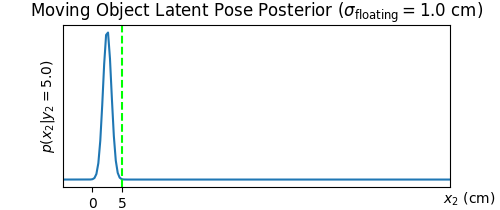
\includegraphics[width=\columnwidth]{outlierModel1a}
  \end{subfigure}%
  \begin{subfigure}[b]{0.5\textwidth}
    \centering
    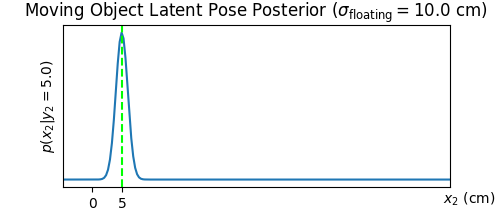
\includegraphics[width=\columnwidth]{outlierModel2a}
  \end{subfigure}
  \begin{subfigure}[b]{0.5\textwidth}
    \centering
    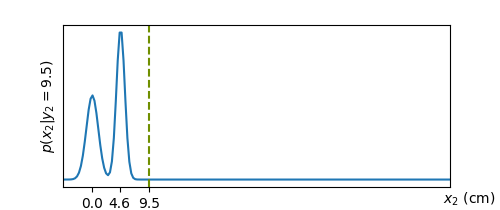
\includegraphics[width=\columnwidth]{outlierModel1b}
  \end{subfigure}%
  \begin{subfigure}[b]{0.5\textwidth}
    \centering
    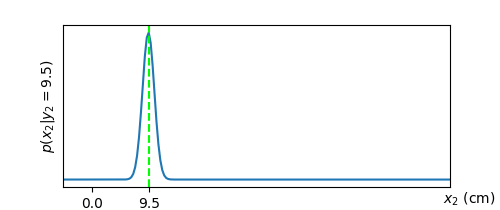
\includegraphics[width=\columnwidth]{outlierModel2b}
  \end{subfigure}
  \begin{subfigure}[b]{0.5\textwidth}
    \centering
    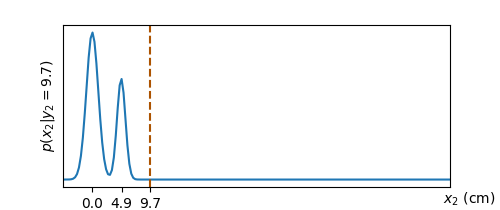
\includegraphics[width=\columnwidth]{outlierModel1c}
  \end{subfigure}%
  \begin{subfigure}[b]{0.5\textwidth}
    \centering
    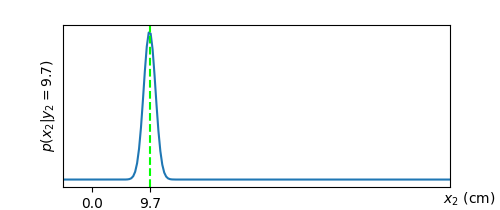
\includegraphics[width=\columnwidth]{outlierModel2c}
  \end{subfigure}
  \begin{subfigure}[b]{0.5\textwidth}
    \centering
    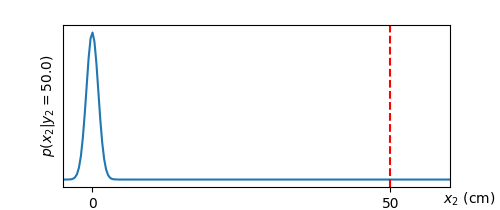
\includegraphics[width=\columnwidth]{outlierModel1d}
    \subcaption{
      Pose posteriors where \\ $\sigma_\mathrm{floating} = \sigma_\mathrm{inlier} = 0.01$.
    }
  \end{subfigure}%
  \begin{subfigure}[b]{0.5\textwidth}
    \centering
    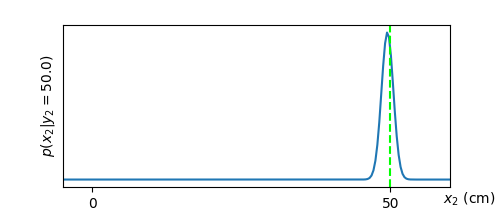
\includegraphics[width=\columnwidth]{outlierModel2d}
    \subcaption{
      Pose posteriors where \\ $\sigma_\mathrm{floating} = 10\sigma_\mathrm{inlier} = 10$ cm.
    }
  \end{subfigure}
  \caption{
    Posteriors over the latent pose of an object $p(x_2 | y_2) = p(x_2 | y_2, x_1 = 0)$, under two different settings of the dynamics parameter.
    The noisy observational model's inlier distribution is given by $\sigma_\mathrm{inlier} = 1$ cm, while the prior probability of an outlier is $p_\mathrm{outlier} = 0.1$.
    The dashed line represents the observed pose $y_2$, with color representing the probability that $y_2$ is an outlier (totally green means $p_\mathrm{inlier} = 1$, while totally red means $p_\mathrm{outlier} = 1$).
  }
  \label{fig:outlierModel}
\end{figure}

\pagebreak

\section{Lessons for improving scene graph priors}
There are two big lessons from these experiments regarding the improvement of the scene graph model.
The first lesson is that the qualitative behavior of the posterior is highly sensitive to the proper tuning of hyperparameters.
As seen in the analysis of the structure posterior, hyperparameter settings had a crucial impact on the performance of the model.
Furthermore, this section showed how introducing dynamics over continuous parameters impacts the posterior probability of a contact edge existing between two objects.
Interactions like these can be highly counter-intuitive, and difficult to explore using synthetic tests like the ones explored here.
It's for these reasons that in future development of scene graph models, training model hyperparameters and analyzing model performance using real-world data will be a vital step in improving accuracy.
The subsequent chapter explores this further, and especially how real-world data can be used to test and improve scene graph models.

The second lesson is the importance of considering how the \textit{relative} concentrations of different component distributions in the model will affect the posterior.
More specifically, the Bayesian Occam's Razor suggests that distributions with very high concentrations of their mass will tend to have an overinflated impact on where mass ends up in the posterior.
In the simplest case, the relative concentration of distributions in different model structures have a large impact on which model structures are more probable in the posterior.
In the extreme case, this can lead to entire parts of the prior model being neglected in favor of assigning high weights to areas that maximize the density of the especially peaky model component.
The proposed scene graph model has a large family of possible model structures, with different continuous parameter distributions of varying concentration and dimension.
\textit{All} of these distributions, and their relative concentration, matter for the calculation of the structure posterior, and thus must be considered \textit{jointly} in order to have a truly accurate understanding of the posterior in the full model.
